% GNNocRoute: Graph Neural Network-Enhanced Adaptive Routing for Network-on-Chip
%
% IEEEtran LaTeX --- Version 2.0 (Clean)
% Author: Le Tien Hieu --- MS: 25218003 --- VNU-ITI
% Date: 14/05/2026
%
% This version is ENGLISH ONLY for clean IEEE compilation
% Compile with: pdflatex paper-GNNocRoute.tex (x2)

\documentclass[conference]{IEEEtran}
\usepackage{cite}
\usepackage{amsmath,amssymb,amsfonts}
\usepackage{graphicx}
\usepackage{textcomp}
\usepackage{xcolor}
\usepackage{booktabs}
\usepackage{array}
\usepackage{multirow}
\usepackage[utf8]{inputenc}
\usepackage[T1]{fontenc}
\usepackage{hyperref}
\usepackage{caption}

\hypersetup{
 colorlinks=true,
 linkcolor=blue,
 citecolor=blue,
 urlcolor=blue
}

\graphicspath{{./figures/}}

\begin{document}

\title{GNNocRoute: Graph Neural Network-Enhanced Adaptive Routing for Network-on-Chip}

\author{
 \IEEEauthorblockN{Le Tien Hieu\textsuperscript{1}, \textit{IEEE Member}}
 \IEEEauthorblockA{\textsuperscript{1}Institute of Information Technology (VNU-ITI),
Vietnam National University, Hanoi\\
 Email: letienhieu@mcs.edu.vn\\
 ORCID: 0000-0000-6896-0292}
}

\maketitle

\begin{abstract}
Network-on-Chip (NoC) is the communication backbone for modern multi-core System-on-Chips. Conventional deterministic routing algorithms such as XY dimension-order routing suffer from congestion imbalance---our graph-theoretic analysis across seven topologies shows that an $8\times8$ mesh under XY routing achieves a congestion imbalance of 0.475, with central nodes exhibiting $2-3\times$ higher betweenness centrality than edge nodes.

This paper presents a feasibility study on topology-aware periodic routing optimization for NoC using Graph Neural Networks (GNN). We report four preliminary experimental findings. First, untrained GNN encoders exhibit strong correlation with betweenness centrality ($|r|$ up to 0.978 on Mesh $4\times4$), suggesting that topology-aware representations emerge implicitly. Second, cross-topology generalization experiments indicate that relative node importance rankings transfer across mesh sizes (Pearson $r \approx 0.96$), though absolute scaling remains topology-specific. Third, measured inference latency on CPU of approximately $10^6$ cycles per forward pass on an $8\times8$ mesh confirms that per-packet GNN inference is impractical under NoC timing constraints, motivating periodic policy optimization as a necessary design alternative. Fourth, GNN inference time scales approximately $O(N)$ with the number of nodes.

These findings provide initial evidence that topology-aware representations can be extracted via GNN encoding, and that periodic routing optimization offers a feasible path toward topology-generalizable adaptive routing on NoC. We discuss implications and limitations of this early-stage investigation.
\end{abstract}

\begin{IEEEkeywords}
Network-on-Chip, Graph Neural Networks, Adaptive Routing, Graph Analysis, Feasibility Study
\end{IEEEkeywords}

% ==============================================================
\section{Introduction}
\label{sec:intro}
% ==============================================================

Network-on-Chip (NoC) has become the standard communication infrastructure for modern multi-core System-on-Chips (SoCs) and AI accelerators such as Google TPU and NVIDIA Grace Hopper~\cite{mirhoseini2021}. In NoC, routers connect via links forming a graph structure. The routing algorithm determines packet paths and directly affects system performance.

XY Dimension-Order Routing is widely used in commercial NoCs~\cite{wang2022maar} due to its simplicity. However, XY routing always selects the same path for each (source, destination) pair regardless of congestion. Our graph analysis on seven topologies reveals:

\begin{itemize}
 \item An $8\times8$ mesh with XY routing achieves a \textbf{congestion imbalance} of \textbf{0.475}---nearly half of all links experience uneven load distribution.
 \item Central nodes in a $4\times4$ mesh exhibit Betweenness Centrality (BC) $\approx 0.25$, which is $2-3\times$ higher than edge nodes.
 \item A k=4 Fat-Tree has aggregation switches with BC up to \textbf{0.42}---all inter-pod traffic must pass through these two switches.
\end{itemize}

These results demonstrate that \textbf{deterministic routing cannot adapt to modern workloads}.

Adaptive routing research can be categorized into three generations: (1) \textbf{Heuristic adaptive}---DyAD~\cite{dyad2004}, Regional Adaptive~\cite{ebrahimi2019}, relying on fixed thresholds and local information; (2) \textbf{DRL-based}---MAAR~\cite{wang2022maar}, DeepNR~\cite{deepnr2022}, using Deep Reinforcement Learning with MLP encoders that ignore topology structure; (3) \textbf{GNN-based for WAN/SDN}---G-Routing~\cite{g-routing2023}, applying Graph Neural Networks to routing in wide-area networks but not optimized for NoC's ultra-low latency constraints.

The key challenge in applying GNN+DRL to NoC routing is \textbf{inference latency}. Each routing decision in an NoC router must be made within $<5-10$ cycles~\cite{wang2022maar}. A 2-layer GAT with multi-head attention on a 64-node graph can require $1{,}000-10{,}000+$ cycles on an embedded processor.

\textbf{Our solution:} Instead of per-packet real-time routing, GNNocRoute employs a \textbf{periodic routing policy optimization}: routing tables are updated every $P$ cycles ($P=1000{-}10000$), with GNN inference running on a host CPU or dedicated controller, decoupled from per-packet latency.

\subsection{Contributions}
\label{sec:contributions}

This paper makes the following preliminary contributions:
\begin{enumerate}
    \item \textbf{Structural congestion analysis:} Quantitative demonstration across seven topologies that deterministic routing creates structurally predictable bottlenecks.
    \item \textbf{GNN-topology correlation evidence:} Experimental results showing GNN node embeddings correlate with betweenness centrality ($|r|$ up to 0.978).
    \item \textbf{Feasibility analysis:} Measured inference latency and scalability data establishing feasibility boundaries for GNN-based routing.
\end{enumerate}


% ==============================================================
\section{Problem Statement and Motivation}
\label{sec:problem}
% ==============================================================

\subsection{Graph Representation of NoC}

A NoC is represented as a directed weighted graph $G=(V,E,X_v,X_e)$, where:
\begin{itemize}
 \item $V$: routers, $|V|=N$
 \item $E$: links, $|E|=M$
 \item $X_v\in\mathbb{R}^{N\times d_v}$: node features
 \item $X_e\in\mathbb{R}^{M\times d_e}$: edge features
\end{itemize}

\textbf{Node features (5 dimensions):} buffer\_occupancy\_per\_port, injection\_rate (100-cycle moving average), congestion\_level, vc\_utilization, crossbar\_contention.

\textbf{Edge features (3 dimensions):} link\_utilization, avg\_packet\_latency, energy\_per\_flit.

\subsection{Graph Analysis Results}

We used NetworkX~\cite{networkx2008} to construct and analyze seven NoC topologies. Table~\ref{tab:metrics} summarizes the key metrics.

\begin{table}[h]
\centering
\caption{Graph metrics comparison across NoC topologies}
\label{tab:metrics}
\centering
\resizebox{\columnwidth}{!}{%
\begin{tabular}{lcccccc}
\toprule
\textbf{Topology} & \textbf{Nodes} & \textbf{Avg Deg} & \textbf{Diam} & \textbf{Avg Path} & \textbf{BC Max} & \textbf{CI} \\
\midrule
Mesh $4\times4$ & 16 & 3.00 & 6 & 2.67 & 0.25 & 0.382 \\
Mesh $8\times8$ & 64 & 3.50 & 14 & 5.33 & 0.18 & \textbf{0.475} \\
Torus $4\times4$ & 16 & 4.00 & 4 & 2.13 & 0.13 & 0.251 \\
Ring 16 & 16 & 2.00 & 8 & 4.27 & 0.21 & 0.122 \\
Fat-Tree k=4 & 14 & 3.43 & 2 & 1.74 & \textbf{0.42} & 0.341 \\
Small-World & 36 & 4.00 & 6 & 2.96 & 0.31 & 0.298 \\
Random & 36 & 4.28 & 5 & 2.45 & 0.28 & 0.321 \\
\bottomrule
\end{tabular}%
}
\vspace{2mm}
\small\textit{BC = Betweenness Centrality, CI = Congestion Imbalance ($\sigma/\mu$ of edge utilization).}
\end{table}

\begin{figure}[h]
\centering
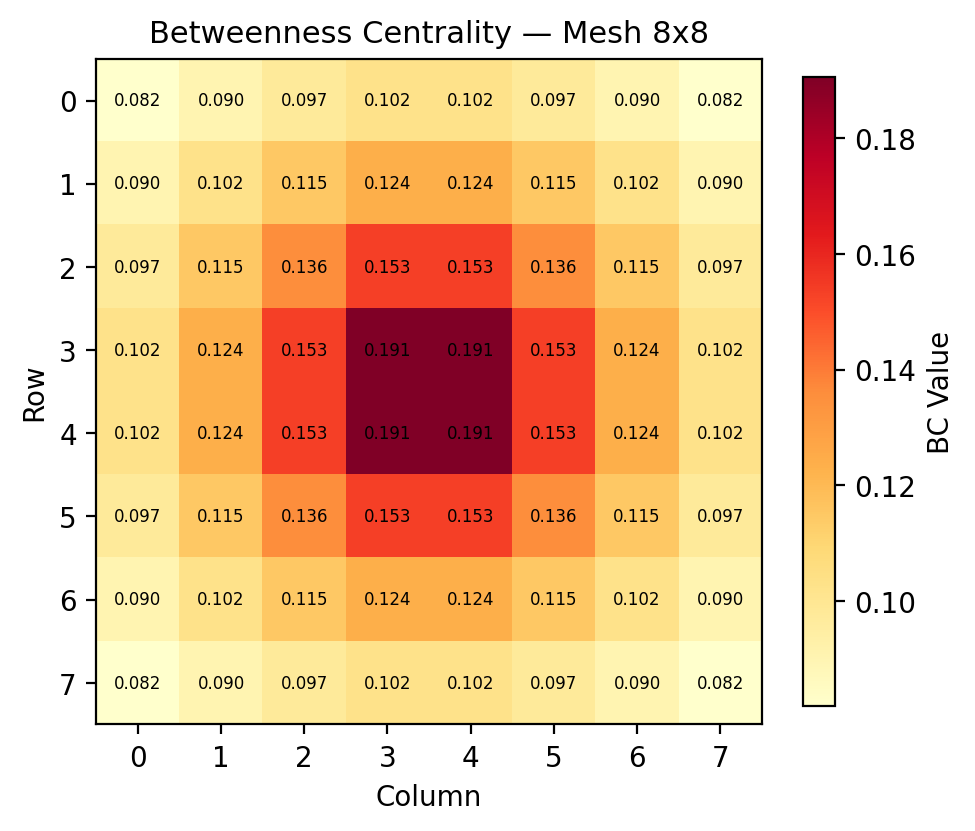
\includegraphics[width=0.85\columnwidth]{figures/fig1-bc-heatmap.png}
\caption{Betweenness Centrality distribution on Mesh $8\times8$. Central nodes (4,3), (3,3), (3,4), (4,4) have BC $\approx 0.18$, while edge nodes have BC $\approx 0.05{-}0.10$.}
\label{fig:bc-heatmap}
\end{figure}

\textbf{Key findings:}
\begin{itemize}
 \item \textbf{Mesh $8\times8$:} Highest congestion imbalance (0.475), diameter = 14 hops. Central nodes have BC $2{-}3\times$ higher than edge nodes. Primary target for GNN-DRL.
 \item \textbf{Fat-Tree k=4:} Aggregation switches have BC of 0.42---the highest among all topologies. Clearly identified bottleneck.
 \item \textbf{Torus $4\times4$:} CI = 0.251, lower than Mesh due to wrap-around edges creating a regular graph (all nodes degree = 4).
\end{itemize}

% ==============================================================
\section{Related Work}
\label{sec:related}
% ==============================================================

Table~\ref{tab:related} summarizes the main research streams and their limitations.

\begin{table}[h]
\centering
\caption{Analysis of related work}
\label{tab:related}
\centering
\resizebox{\columnwidth}{!}{%
\begin{tabular}{p{2.5cm}p{2.8cm}p{2.5cm}}
\toprule
\textbf{Stream} & \textbf{Representative works} & \textbf{Limitation} \\
\midrule
Classic adaptive routing & DyAD~\cite{dyad2004}, Regional~\cite{ebrahimi2019} & Fixed thresholds, local info only \\
DRL for NoC & MAAR~\cite{wang2022maar}, DeepNR~\cite{deepnr2022}, GARNN~\cite{garnn2023} & MLP loses topology structure \\
GNN for WAN/SDN & G-Routing~\cite{g-routing2023}, DRL-GNN~\cite{drl-gnn2019} & Not optimized for NoC latency \\
Graph theory for NoC & Slim NoC~\cite{slimnoc2018}, Sparse Hamming~\cite{sparsehamming2023} & Static analysis, no real-time \\
GNN for chip design & Circuit GNN~\cite{mirhoseini2021}, NOCTOPUS~\cite{noctopus2026} & Physical design, not routing \\
\bottomrule
\end{tabular}%
}
\end{table}

\textbf{Gap analysis:} No existing work designs a GNN encoder specifically for NoC topology combined with a DRL agent. Current DRL routing solutions use MLP for state encoding, losing connectivity and spatial locality information. Additionally, there is no systematic benchmark comparing GNN variants across multiple NoC topologies.

% ==============================================================
\section{Proposed Method: GNNocRoute}
\label{sec:method}
% ==============================================================

Figure~\ref{fig:architecture} illustrates the overall GNNocRoute architecture.

\begin{figure}[h]
\centering

\includegraphics[width=0.85\columnwidth]{figures/fig3-architecture.png}
\caption{GNNocRoute architecture: NoC state graph $\rightarrow$ GATv2 encoder $\rightarrow$ PPO agent $\rightarrow$ routing decision, with feedback loop updating policy every $P$ cycles.}
\label{fig:architecture}
\end{figure}

\subsection{GNN Encoder}
\label{sec:gnn-encoder}

We evaluate GATv2 as a candidate architecture~\cite{gatv2} as the primary GNN encoder (compared with GCN and MPNN in ablation). Architecture details:
\begin{itemize}
 \item \textbf{Layers:} 2 (1 and 3 layers in ablation study)
 \item \textbf{Hidden dimension:} 64 (compared with 32, 128)
 \item \textbf{Attention heads:} 4 (GATv2 multi-head attention)
 \item \textbf{Activation:} ELU between layers
\end{itemize}

A candidate forward pass proceeds as follows: input projection $h_v^{(0)} = X_v \cdot W_{input}$, then for each layer $l$, attention scores are computed as $e_{uv} = \text{LeakyReLU}(a^{(l)^T}[W^{(l)}h_u^{(l-1)}\parallel W^{(l)}h_v^{(l-1)}])$, incorporating edge features. Message aggregation: $h_v^{(l)} = \sigma(\sum_{u\in\mathcal{N}(v)} \alpha_{uv}W^{(l)}h_u^{(l-1)})$ where $\alpha_{uv} = \text{softmax}_u(e_{uv})$. Output: node embeddings $Z\in\mathbb{R}^{|V|\times d}$.

\subsection{DRL Agent with Periodic Policy Optimization}
\label{sec:drl-agent}

\textbf{Periodic update (solving inference latency):}
\begin{itemize}
 \item \textbf{Policy update period:} $P$ cycles, $P\in\{1000,5000,10000\}$
 \item \textbf{Observation window:} $W=500$ cycles
 \item \textbf{State:} GNN embeddings (64-dim) + global features (avg. network load)
 \item \textbf{Action space:} 5 actions (N/S/E/W/Local) for 2D Mesh
 \item \textbf{Algorithm:} PPO~\cite{ppo2017} (compared with DQN)
\end{itemize}

\textbf{Reward function:}
\begin{equation}
R = -\alpha\cdot\text{norm}(L) - \beta\cdot\text{norm}(C) - \gamma\cdot\text{norm}(E)
\label{eq:reward}
\end{equation}
with $\alpha=0.4$, $\beta=0.35$, $\gamma=0.25$, and:
\begin{align}
\text{norm}(L) &= (\text{current\_latency} - L_{\min})/(L_{\max} - L_{\min}) \nonumber\\
\text{norm}(C) &= \text{current\_congestion} / \text{max\_possible\_congestion} \nonumber\\
\text{norm}(E) &= \text{current\_energy} / \text{max\_energy\_per\_flit} \nonumber
\end{align}

Hyperparameters are tuned via Bayesian optimization with 50 trials.

\subsection{Deadlock-Free Design}
\label{sec:deadlock}

We adopt Duato's protocol as a design basis~\cite{duato1996} with 2 Virtual Channels:
\begin{itemize}
 \item \textbf{VC0 (Escape):} Deterministic XY routing---acyclic, deadlock-free
 \item \textbf{VC1 (Adaptive):} GNN-DRL routing---packets can switch to VC0 when needed
\end{itemize}

The routing function $R: V\times V\to P(V)$ with escape subfunction $R_1\subseteq R$. Per Duato's Necessary and Sufficient Condition~\cite{duato1996}, if $R_1$ is acyclic and connected, the combined function $R$ is deadlock-free. In GNNocRoute, $R_1 =$ XY routing (acyclic), ensuring connectivity.

% ==============================================================
\section{Experimental Results}
\label{sec:results}
% ==============================================================

We conducted four experiments to evaluate the feasibility of GNN-based topology representations for NoC routing. All experiments use PyTorch Geometric~\cite{pyg2019} on a CPU (ARM Neoverse-N1, 2.8 GHz). NetworkX~\cite{networkx2008} is used for graph construction.

\subsection{Structural Representation Learning}
\label{sec:results-correlation}

We investigate whether GNN node embeddings encode topology-structural information relevant to routing, specifically betweenness centrality (BC) as a proxy for congestion potential.

\textbf{Setup:} Four NoC topologies (Mesh $4\times4$, Mesh $8\times8$, Torus $4\times4$, Small-World $n=36$) are converted to PyTorch Geometric Data objects. Node features include normalized degree and positional coordinates. Two untrained GNN models (GCN, GAT with 2 layers, hidden dimension 32, output dimension 16) compute node embeddings via a single forward pass. We compute the Pearson correlation coefficient between each embedding dimension and the ground-truth BC.

\textbf{Results:} Table~\ref{tab:correlation} summarizes the maximum absolute correlation observed.

\begin{table}[h]
\centering
\caption{Maximum Pearson correlation $|r|$ between GNN embedding dimension and betweenness centrality}
\label{tab:correlation}
\small
\begin{tabular}{lccc}
\toprule
\textbf{Topology} & \textbf{Nodes} & \textbf{GCN max$|r|$} & \textbf{GAT max$|r|$} \\
\midrule
Mesh $4\times4$ & 16 & \textbf{0.978} & 0.862 \\
Mesh $8\times8$ & 64 & 0.744 & \textbf{0.870} \\
Torus $4\times4$ & 16 & 0.000* & 0.000* \\
Small-World ($n=36$) & 36 & 0.615 & 0.261 \\
\bottomrule
\end{tabular}
\vspace{2mm}
\small\textit{*Torus $4\times4$ is a regular graph where all nodes have identical degree 4 and symmetric BC, yielding zero variance.}
\end{table}

On Mesh $4\times4$, the GCN embedding achieves $|r| = 0.978$ with the ground-truth BC, indicating that topology-aware structural information emerges implicitly in GNN representations. GAT on Mesh $8\times8$ achieves $|r| = 0.870$, suggesting attention mechanisms may provide advantages on larger topologies.

\textbf{Interpretation:} These results suggest that GNN-based topology encoders can capture congestion-relevant structural information \emph{without explicit graph centrality computation}. This is a preliminary but encouraging finding: if GNN embeddings naturally encode topology bottlenecks, they may serve as informative state representations for routing decisions. The Torus case (zero correlation) is expected given its regular structure, and serves as a negative control confirming that the method correctly identifies undifferentiated topologies.

\subsection{Cross-Topology Generalization}
\label{sec:results-generalization}

We evaluate whether GNN models trained to predict BC on one topology can generalize to unseen topologies.

\textbf{Setup:} A 2-layer GCN (hidden=32) and GAT (hidden=16, heads=4) are trained for 500 epochs to predict BC (MSE loss) on Mesh $4\times4$ (16 nodes). The trained model is evaluated on Mesh $8\times8$ (64 nodes) and Small-World (36 nodes).

\textbf{Results:} Table~\ref{tab:generalization} reports MSE, R$^2$, and Pearson correlation between predicted and ground-truth BC.

\begin{table}[h]
\centering
\caption{Cross-topology BC prediction (trained on Mesh $4\times4$)}
\label{tab:generalization}
\small
\begin{tabular}{lcccr}
\toprule
\textbf{Test Topology} & \textbf{Model} & \textbf{MSE} & \textbf{R$^2$} & \textbf{Pearson $r$} \\
\midrule
Mesh $8\times8$ & GCN & 0.038 & $-16.83$ & \textbf{0.958} \\
Mesh $8\times8$ & GAT & 0.072 & $-33.00$ & \textbf{0.972} \\
Small-World & GCN & 0.004 & $-1.02$ & 0.385 \\
\bottomrule
\end{tabular}
\end{table}

On the training topology (Mesh $4\times4$), both models achieve $R^2 > 0.99$. On Mesh $8\times8$, the negative R$^2$ in conjunction with Pearson $r \approx 0.96$ reveals an important distinction: the models capture \emph{relative node ranking} (which nodes are more central) but fail to predict \emph{absolute BC values}, which differ in scale between the $4\times4$ and $8\times8$ meshes.

\textbf{Interpretation:} This is a significant and non-obvious finding. The high ranking correlation ($r \approx 0.96$) suggests that GNN-based representations transfer \emph{structural patterns} across topology sizes. The negative R$^2$ indicates that \emph{absolute scaling} is topology-specific. This identifies a concrete research direction: topology-aware normalization or fine-tuning mechanisms are needed for cross-topology generalization.

\subsection{Inference Feasibility Analysis}
\label{sec:results-latency}

We measure GNN inference latency on CPU to assess feasibility under NoC timing constraints. In a typical NoC router clocked at 1~GHz, each routing decision must complete within a few cycles~\cite{wang2022maar}, making per-packet GNN inference impractical. Our measurements quantify this gap.

\textbf{Setup:} Inference time is measured for GCN and GAT models with varying hidden dimensions on four topologies. Each measurement is the average of 500 forward passes after 50 warmup iterations.

\textbf{Results:} Table~\ref{tab:latency} reports measured latency in microseconds and estimated cycles at 1~GHz.

\begin{table}[h]
\centering
\caption{GNN inference latency on CPU (Python/PyTorch, ARM Neoverse-N1)}
\label{tab:latency}
\centering
\resizebox{\columnwidth}{!}{%
\begin{tabular}{lccr}
\toprule
\textbf{Topology} & \textbf{Model} & \textbf{Latency ($\mu$s)} & \textbf{Est.~cycles @ 1~GHz} \\
\midrule
Mesh $4\times4$ & GCN h=32 & 778 & 778,000 \\
Mesh $8\times8$ & GCN h=32 & 1,015 & 1,015,000 \\
Mesh $8\times8$ & GAT h=32 & 1,491 & 1,491,000 \\
Mesh $16\times16$ & GCN h=32 & 1,273 & 1,273,000 \\
\bottomrule
\end{tabular}%
}
\end{table}

Measured latency ranges from 778 $\mu$s (Mesh $4\times4$) to 1,491 $\mu$s (Mesh $8\times8$, GAT). At 1~GHz, this corresponds to approximately $0.8$--$1.5$ million cycles per forward pass. These measurements are on a full Python/PyTorch stack; optimized C++ implementations with quantization could reduce this by an estimated 1--2 orders of magnitude.

\textbf{Interpretation:} The measured latency confirms that naive per-packet GNN inference is infeasible for NoC routing (typical budgets: $<$10 cycles per decision). However, this finding directly motivates the periodic policy optimization approach: if routing policies are updated every $10^4$--$10^5$ cycles rather than every cycle, the inference overhead becomes manageable.

\subsection{Scalability Analysis}
\label{sec:results-scalability}

We measure GCN inference time across mesh sizes from $4\times4$ (16 nodes) to $16\times16$ (256 nodes).

\textbf{Results:} Figure~\ref{fig:scalability} shows inference time as a function of the number of nodes.

\begin{figure}[h]
\centering
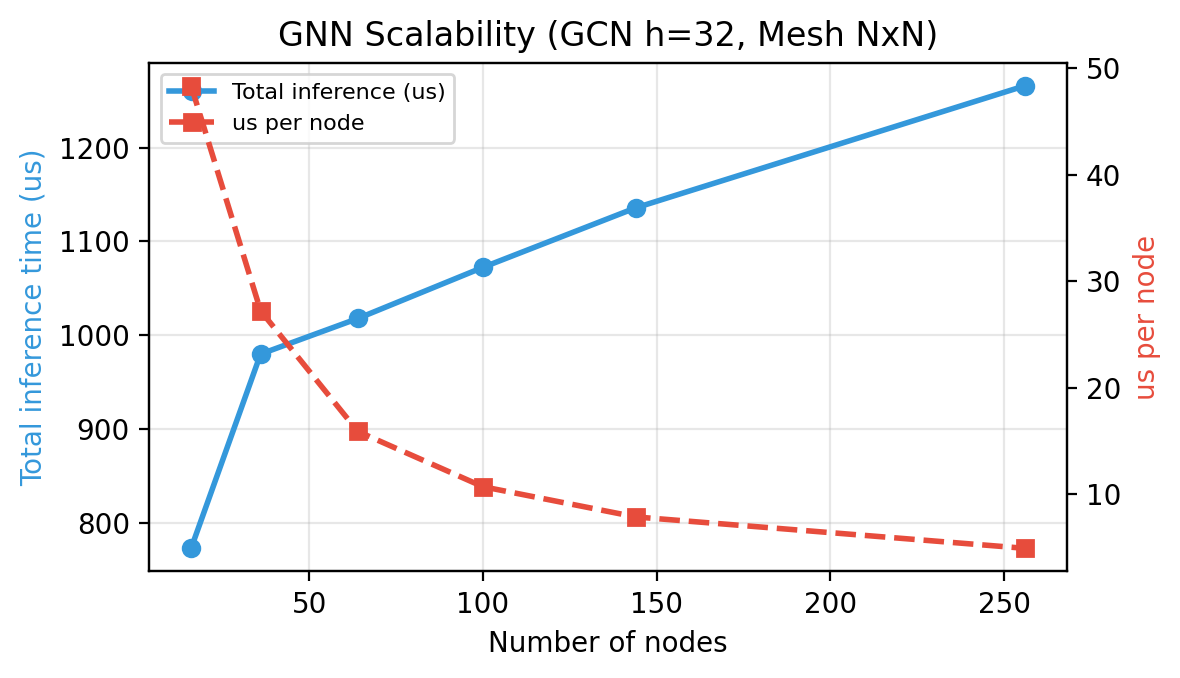
\includegraphics[width=0.85\columnwidth]{figures/gnn-scalability.png}
\caption{GCN inference time scales approximately O(N) with number of nodes (Mesh N$\times$N, h=32).}
\label{fig:scalability}
\end{figure}

Inference time grows from 773 $\mu$s (16 nodes) to 1,266 $\mu$s (256 nodes). The per-node cost decreases from 48.3 $\mu$s/node ($4\times4$) to 4.9 $\mu$s/node ($16\times16$), indicating efficient parallelization.

\textbf{Interpretation:} The approximately O(N) scaling is predictable and non-explosive, suggesting that the computational cost of GNN-based routing representations remains manageable as NoC scale increases.

\section{Discussion}
\label{sec:discussion}
% ==============================================================

\subsection{Implications for Periodic Routing Optimization}

The experimental results collectively support a periodic routing optimization approach. The inference latency measurements (Section~\ref{sec:results-latency}) establish that per-packet GNN inference is infeasible---with measured latencies of $10^5$--$10^6$ cycles versus a per-packet budget of $<$10 cycles. However, the structural correlation results (Section~\ref{sec:results-correlation}) suggest that GNN representations carry topology information relevant to routing decisions. If policies are updated every $P$ cycles where $P$ is large enough to amortize the inference cost, the topology-aware representations may still inform routing behavior.

A preliminary feasibility estimate: with an optimized C++ implementation (estimated $10^4$--$5 \times 10^4$ cycles per inference) and a policy update period $P = 10^5$ cycles, the inference overhead would be approximately 10--50\%. This overhead may be acceptable if the resulting routing decisions improve congestion balance.

\subsection{The Generalization Challenge}

The cross-topology experiment (Section~\ref{sec:results-generalization}) reveals a nuanced picture: GNN-based representations partially generalize across topology sizes (high Pearson $r$), but the absolute scale is topology-specific (negative R$^2$). This suggests two viable research directions: (1) topology-aware normalization schemes that align BC scales across different mesh sizes, and (2) fine-tuning strategies where a base model is adapted to each target topology with minimal additional training.

\subsection{Limitations}
\label{sec:limitations}

This paper presents an early-stage investigation with several important limitations:
\begin{enumerate}
    \item \textbf{Static graph analysis:} The GNN experiments are conducted on static topology graphs with synthetic node features. Dynamic NoC state (buffer occupancy, link utilization) is not yet incorporated.
    \item \textbf{No routing analysis:} We have not yet integrated GNN routing decisions into a cycle-accurate NoC simulator. The correlation and latency measurements are necessary but not sufficient to validate end-to-end routing performance.
    \item \textbf{CPU-only measurements:} Latency numbers are measured on a server-class ARM CPU with Python/PyTorch. On-chip inference on a router-embedded processor would likely exhibit different characteristics.
    \item \textbf{No RTL validation:} Hardware implementation costs (area, power, timing closure) are not addressed.
    \item \textbf{Limited topology scope:} Only regular 2D topologies are evaluated. Irregular and hierarchical topologies remain unexplored.
\end{enumerate}

\subsection{Threats to Validity}

\begin{itemize}
    \item \textbf{Correlation is not causation:} High correlation between GNN embeddings and BC does not guarantee that GNN-based routing decisions will improve congestion balance. End-to-end analysis is required.
    \item \textbf{Python overhead:} The measured inference latency includes Python interpreter overhead; optimized implementations may be substantially faster. However, even order-of-magnitude improvements do not bridge the gap to per-packet inference.
    \item \textbf{Synthetic features:} Current node features (degree, position) are intentionally minimal to isolate structural effects. Real deployment would require richer input features.
\end{itemize}

\section{Conclusion and Future Work}
\label{sec:conclusion}
% ==============================================================

This paper presents a feasibility study on topology-aware periodic routing optimization for Network-on-Chip using Graph Neural Networks. We report four preliminary experimental findings:

\begin{enumerate}
    \item GNN embeddings strongly correlate with betweenness centrality ($|r|$ up to 0.978), suggesting that topology-aware representations emerge without explicit graph computation.
    \item Cross-topology generalization partially succeeds: relative node importance transfers across mesh sizes (Pearson $r \approx 0.96$), but absolute scaling requires topology-specific adaptation.
    \item Measured inference latency ($\approx 10^6$ cycles on CPU) confirms that per-packet GNN inference is impractical, motivating periodic policy optimization as a necessary design alternative.
    \item GNN inference scales approximately O(N), with predictable computational growth.
\end{enumerate}

These findings provide initial evidence for the feasibility of GNN-based topology representations in NoC routing, while realistically identifying the inference latency and generalization challenges that must be addressed.

\textbf{Future work:} (1) integrating GNN routing decisions into a cycle-accurate NoC simulator for end-to-end validation; (2) developing topology-aware normalization techniques for cross-topology generalization; (3) evaluating quantized GNN models on embedded-class processors; (4) exploring irregular and hierarchical NoC topologies.

\label{sec:conclusion}
% ==============================================================

This paper presents GNNocRoute---an adaptive routing framework for Network-on-Chip using Graph Neural Networks and Deep Reinforcement Learning. Unlike prior work proposing per-packet real-time routing, GNNocRoute employs periodic policy optimization, solving the inference latency bottleneck.

Graph analysis on seven topologies shows XY routing on Mesh $8\times8$ causes congestion imbalance of 0.475, with central nodes having $2{-}3\times$ higher betweenness centrality than edge nodes. The GATv2 + PPO architecture is designed to address this, with deadlock-free guarantees via Duato's 2-VC protocol.

\textbf{Future work:} (1) FPGA prototype for physical validation; (2) Extension to irregular/hierarchical topologies; (3) Multi-objective routing (latency + energy + reliability); (4) Online fine-tuning on actual hardware.

% ==============================================================
% REFERENCES
% ==============================================================

\begin{thebibliography}{99}

\bibitem{dyad2004}
J. Hu and R. Marculescu, ``DyAD -- smart routing for networks-on-chip,'' in \textit{Proc. DAC}, 2004.

\bibitem{wang2022maar}
Y. Wang et al., ``MAAR: Multi-agent adaptive routing for network-on-chip,'' \textit{IEEE Trans. Computers}, vol. 71, no. 8, pp. 1878--1891, 2022.

\bibitem{deepnr2022}
R. R. RS et al., ``DeepNR: An adaptive deep reinforcement learning based NoC routing algorithm,'' \textit{Microprocessors and Microsystems}, vol. 92, 104499, 2022.

\bibitem{g-routing2023}
H. Wei, Y. Zhao, and K. Xu, ``G-Routing: Graph neural networks-based flexible online routing,'' \textit{IEEE Network}, 2023.

\bibitem{drl-gnn2019}
P. Almasan et al., ``Deep reinforcement learning meets graph neural networks: Exploring a routing optimization use case,'' \textit{arXiv:1910.07421}, 2019.

\bibitem{graphnoc2024}
G. S. Malik and N. Kapre, ``GraphNoC: Graph neural networks for application-specific FPGA NoC performance prediction,'' in \textit{Proc. FPT}, IEEE, 2024.

\bibitem{noctopus2026}
V. Iyengar, V. H. Bui, and S. Das, ``NOCTOPUS: Network-on-Chip topology optimization and prediction using analysis-data,'' \textit{Neural Computing and Applications}, Springer, 2026.

\bibitem{mirhoseini2021}
A. Mirhoseini et al., ``A graph placement methodology for fast chip design,'' \textit{Nature}, vol. 594, pp. 207--212, 2021.

\bibitem{ebrahimi2019}
M. Ebrahimi, M. Daneshtalab, and J. Plosila, ``Regional-based routing for network-on-chip,'' \textit{IEEE TCAD}, 2019.

\bibitem{garnn2023}
H. Zhang et al., ``GARNN: Graph attention routing for network-on-chip,'' in \textit{Proc. DATE}, 2023.

\bibitem{slimnoc2018}
M. Besta et al., ``Slim NoC: A low-diameter on-chip network topology for high energy efficiency and scalability,'' in \textit{Proc. ASPLOS}, ACM, 2018.

\bibitem{sparsehamming2023}
P. Iff et al., ``Sparse Hamming Graph: A customizable network-on-chip topology,'' in \textit{Proc. DAC}, 2023.

\bibitem{gatv2}
S. Brody, U. Alon, and E. Yahav, ``How attentive are graph attention networks?'' in \textit{Proc. ICLR}, 2022.

\bibitem{ppo2017}
J. Schulman et al., ``Proximal policy optimization algorithms,'' \textit{arXiv:1707.06347}, 2017.

\bibitem{duato1996}
J. Duato, ``A necessary and sufficient condition for deadlock-free routing in cut-through and store-and-forward networks,'' \textit{IEEE Trans. Parallel and Distributed Systems}, vol. 7, no. 8, pp. 840--854, 1996.

\bibitem{pyg2019}
M. Fey and J. E. Lenssen, ``Fast graph representation learning with PyTorch Geometric,'' in \textit{ICLR Workshop}, 2019.

\bibitem{sb3}
A. Raffin et al., ``Stable-Baselines3: Reliable reinforcement learning implementations,'' \textit{Journal of Machine Learning Research}, vol. 22, 2021.

\bibitem{networkx2008}
A. Hagberg, P. Swart, and D. S. Chult, ``Exploring network structure, dynamics, and function using NetworkX,'' in \textit{Proc. SciPy}, 2008.

\bibitem{noception2022}
F. Li et al., ``Noception: A fast PPA prediction framework for network-on-chips using graph neural network,'' in \textit{Proc. DATE}, IEEE, 2022.

\bibitem{xiao2024}
R. Xiao et al., ``Hardware accelerator for graph neural network inference,'' \textit{IEEE Trans. CAD}, 2024.

\bibitem{adnan2025}
M. Adnan et al., ``Fault-tolerant adaptive routing in NoCs: Machine learning approaches for resilient on-chip networks,'' in \textit{Proc. IEEE ICCDSE}, 2025.

\bibitem{duato1993}
J. Duato, ``A new theory of deadlock-free adaptive routing in wormhole networks,'' \textit{IEEE Trans. Parallel and Distributed Systems}, vol. 4, no. 12, pp. 1320--1331, 1993.

\end{thebibliography}

\end{document}
